\documentclass[10pt,a4paper]{article}
\usepackage{amsmath,amssymb,amsthm,graphicx}
\usepackage{amsmath,amssymb,amsthm,graphicx,tikz,enumitem}
\newcommand{\Search}{\mathsf{Search}}
\newcommand{\Flow}{\mathsf{Flow}}
\newcommand{\supp}{\operatorname{supp}}
\newcommand{\st}{\operatorname{st}}
\newcommand{\en}{\operatorname{en}}
\newcommand{\of}{\operatorname{of}}
\newcommand{\joint}{\mathbin{\dot\cup}}
\newenvironment{result}[1]{\par\medskip\noindent\textbf{#1.}\itshape}{\par\medskip}
\allowdisplaybreaks
\title{Exponential lower bounds for bounded-repetition semantic branching programs solving amplified Flow search formulas}
\author{Anastasia Sofronova, Dmitry Sokolov}
\date{doi:10.4230/LIPIcs.CCC.2021.17; CC BY 4.0}
\begin{document}
\maketitle
\noindent\textit{Editorial note.} Faithful editable transcription of complete formal CC BY main lower-bound proof and all required deferredAppendicesA/B. Original source numbering and page locators retained. Non-bearing introductory proof-plan repetition omitted; all actual construction, induction, cases, equations and deferred proofs retained. Standard mixing and max-flow background cited without recursively re-proving. Original schematicFigures2–4 preserved as extracted image assets; Figure1 parallel-path diagram rendered editably without changing labels. Author mathematical wording, index conventions and printed signs retained, without mathematical corrections or added arguments. All production/extraction/validation solely on Yupeng.\par\medskip
\noindent\textit{Allowed standard prerequisites (editorial).}\begin{itemize}
\item Boolean CNF search, semantic/syntactic branching programs, expander mixing and Max-Flow Min-Cut. Complete source-local restrictions, proper/generalized assignments, Flow encoding, expansion conventions and bearingLemma8/Corollary11/Proposition12 included; standard cited Mixing/Flow-Cut theorems not recursively reproved
\end{itemize}\medskip
\section*{Original search, assignment and branching-program definitions (pp.17:2,17:4--6)}
Consider a search problem, defined by a relation $S\subseteq I\times O$ for some finite sets $I$ and $O$. On input $x\in I$ the search problem is to find some output in $S(x):=\{o\in O\mid(x,o)\in S\}$.
\begin{result}{Definition 1}
A unsatisfied search problem $\Search_\varphi$ for an unsatisfiable CNF formula $\varphi:=\bigwedge_{i\in I}C_i$ on $n$ variables is defined as follows:
\begin{itemize}\item input: an $n$-variable assignment $z\in\{0,1\}^n$;
\item output: an element $i\in I$ such that clause $C_i$ of $\varphi$ is falsified by $z$.\end{itemize}
\end{result}
Let $X$ be a set of boolean variables. For a variable $x\in X$ we denote $x^1:=x$ and $x^0:=\neg x$.
We say that $\alpha:X\to\{0,1,*,?\}$ is a generalized partial assignment and $\alpha$ assigns or touches $x\in X$ iff $\alpha(x)\in\{0,1,?\}$. And an assignment $\gamma$ is an instance of $\alpha$ iff:
\begin{itemize}\item $\alpha(x)\in\{0,1,*\}$ implies $\gamma(x)=\alpha(x)$;
\item $\alpha(x)=?$ implies $\gamma(x)\in\{0,1\}$.\end{itemize}
If $\alpha$ and $\beta$ are two partial assignments to variables from the set $X$, we say that a generalized partial assignment $\alpha\joint\beta:X\to\{0,1,*,?\}$ is a joint assignment iff:
\begin{itemize}\item if $\alpha(x)=a$ and $\beta(x)\in\{a,*\}$, then $(\alpha\joint\beta)(x)=a$;
\item if $\beta(x)=a$ and $\alpha(x)\in\{a,*\}$, then $(\alpha\joint\beta)(x)=a$;
\item if $\alpha(x)=a$ and $\beta(x)=1-a$, then $(\alpha\joint\beta)(x)=?$;
\item if $\alpha(x)=\beta(x)=*$, then $(\alpha\joint\beta)(x)=*$,
\end{itemize}
where $a\in\{0,1\}$.
\begin{result}{Theorem 4 (Max-Flow Min-Cut [8])}
Let $G:=(V,E)$. For any $s,t\in V$ the maximum value of an $s$-$t$ flow is equal to the minimum capacity over all $s$-$t$ cuts.
\end{result}
Let $X:=\{x_1,\ldots,x_n\}$ be a set of propositional variables and $O$ be a finite set. A branching program is a directed acyclic graph with one source. Every vertex of the graph is labeled by a variable from $X$, or by an element of the set $O$ with respect to the following properties:
\begin{itemize}\item if a vertex is labeled by $o\in O$, then it is a sink;
\item if a vertex is labeled by a variable, then it has exactly two outgoing edges: one edge is labeled by $0$ and the other one is labeled by $1$.\end{itemize}
Every branching program $B$ defines a function $f_B:\{0,1\}^n\to O$. We assume that every input $z\in\{0,1\}^n$ induces a path from source to sink in a natural way. If this path ends in a vertex with a label $o\in O$ then we define $f_B(z):=o$.
We say that $B$ is a branching program for the relation $S\subseteq\{0,1\}\times O$ iff $f_B$ is consistent with $S$: namely if $f_B(z)=o$ then $(z,o)\in S$.
Let $D$ be a branching program and $v$ is a node in it. The subprogram of $D$ with the root $v$ we denote by $D(v)$ and define as a subgraph of $D$ that is reachable from $v$. Also for a partial assignment $\rho$ we define a branching program $D|_\rho$ as the following transformation applied to $D$:
\begin{itemize}\item for each variable $y$ to which $\rho$ assigns a value $a$, contract edges $y=a$ and delete edges $y=\neg a$;
\item delete all vertices that are unreachable from the root.\end{itemize}
These operations only decrease the size of the program.
If $p$ is a consistent path in a branching program, we denote a partial assignment that corresponds to this path by $\tau_p$.
\begin{result}{Definition 5}
Let $B$ be a branching program. We say that $B$ is a (syntactic) read-once branching program or $1$-BP iff on every path from the source to a sink we can see each variable at most once.
We say that $B$ is a $(1,+k)$-BP iff on every path $p$ from the source to a sink there is a set of variables $X_p$ of size at most $k$ such that all other variables appear in $p$ at most once.
And we can twist this definition a little bit and say that $B$ is a semantic $(1,+k)$-BP iff on every consistent path from $p$ source to sink there is a set of variables $X_p$ of size at most $k$ such that all other variables appear in $p$ at most once.
\end{result}
\begin{result}{Lemma 8}
Let $D$ be a $(1,+k)$-BP for $\Search_\varphi$, $p$ be a consistent path from the root to some node $v$. If $p$ has a variable $x$ queried more than one time on it then $D(v)|_{\tau_p}$ is a $(1,+(k-1))$-BP for the $\Search_{\varphi|_{\tau_p}}$. The result holds for both: semantic and syntactic models.
\end{result}
\begin{proof}
A program $D(v)|_{\tau_p}$ is a program for the $\Search_{\varphi|_{\tau_p}}$ by the correctness of the program $D$. Consider a path $s$ in $D$ from $v$ to some leaf. Let $X_s$ be a set of variables that are queried more than one time on $s$. If $|X_s|=k$ and $x\notin X_s$, the path $ps$ has at least $k+1$ variables that are queried more that one time. This is a contradiction. If $|X_s|=k$ and $x\in X_s$, note that in $D(v)|_{\tau_p}$ we contract all edges that correspond to the $x$ variable and hence we transform this path into a path with at most $k-1$ repetitions.
\end{proof}
\section*{Original Section 3: Expanders (pp.17:6--7)}
We are given a graph $G:=(V,E)$. For two subsets of vertices $A,B$ we write $E(A,B)$ to denote the set of pairs $(v,e)$ where $v\in A$, $e$ is an edge that is incident to $v$ and $e$ connects $v$ with some vertex in $B$. We will think about it as about set of edges between $A$ and $B$, but if $A$ and $B$ intersect we count edges within intersection twice. We also use a shortcut notations $E(S):=E(S,V)$ and $\overline S:=V\setminus S$. If the graph we consider is unclear from the context we specify it as a subscript: $E_G(A,B)$.
\begin{result}{Remark 9}
Assuming that $G$ is $\Delta$-regular graph this definition allows us to use natural equalities:
\[|E(S)|=\Delta|S|;\qquad |E(A,\overline A)|=\Delta|A|-|E(A,A)|.\]
\end{result}
We write $N_G(v)$ to denote the set of neighbours of $v$ in the graph $G$. We extend this notion to sets and denote by $N_G(S):=\{v\mid\exists u\in S,(u,v)\in E\}$ the neighbourhood of a set of vertices $S\subseteq V$.
A graph $G:=(V,E)$ is an $(n,\Delta,\alpha)$-algebraic expander (or just expander), if:
\begin{itemize}\item $|V|=n$;
\item the degree of any vertex $v\in V$ equals $\Delta$;
\item the absolute value of the second largest eigenvalue of the adjacency matrix of $G$ is at most $\alpha\Delta$.\end{itemize}
\begin{result}{Lemma 10 (Mixing Lemma [4])}
Let $G:=(V,E)$ be an $(n,\Delta,\alpha)$-expander. For any two subsets $A,B\subseteq V$ the following holds:
\[\left||E(A,B)|-\frac{\Delta|A||B|}{n}\right|\le\alpha\Delta\sqrt{|A||B|}.\]
\end{result}
We also need combinatorial edge expansion. We say that $G:=(V,E)$ satisfies $(r,\beta)$-(edge) expansion property for some $r,\beta>0$, if for all $S\subseteq V$ of size at most $r$ holds $E(S,\overline S)\ge\beta\Delta|S|$. The Mixing Lemma says that any expander graph satisfies expansion property for suitable parameters.
\begin{result}{Corollary 11}
If $G:=(V,E)$ is an $(n,\Delta,\alpha)$-expander, then for any $0<\beta<1-\alpha$ the graph $G$ satisfy $((1-\alpha-\beta)n,\beta)$-expansion property.
\end{result}
\begin{proof}
Consider some $A\subseteq V$ of size at most $(1-\alpha-\beta)n$. Note that $|E(A,\overline A)|=\Delta|A|-|E(A,A)|$. By Mixing Lemma:
\[|E(A,A)|\le\frac{\Delta|A|^2}{n}+\alpha\Delta|A|=\Delta|A|\left(\frac{|A|}{n}+\alpha\right)\le\Delta|A|(1-\beta).\]
Hence $|E(A,\overline A)|\ge\beta\Delta|A|$ by Remark 9.
\end{proof}
The ``vertex analog'' of the next proposition is well known in the literature (for example [9]). We turn it into edge version.
\begin{result}{Proposition 12}
Let $G:=(V,E)$ be a graph of degree $\Delta$. If $G$ satisfies $(r,\beta)$-expansion property then for any set $S\subseteq V$ of size $k\le r$ there is an enumeration $v_1,v_2,\ldots,v_k\in S$ and a sequence $R_1,\ldots,R_k\subseteq E(S)$ such that:
\[R_i=E(\{v_i\},V\setminus\{v_1,v_2,\ldots,v_i\});\qquad |R_i|\ge\beta\Delta.\]
\end{result}
\begin{proof}
We create this sequence in reversed order. Since $|S|\le r$, it holds that $|E(S,\overline S)|\ge\beta\Delta|S|$ and there is a vertex $v_k\in S$ such that $|E(\{v_k\},\overline S)|\ge\beta\Delta$. Let $R_k:=|E(\{v_k\},\overline S)|$, and repeat the process for $S\setminus\{v_k\}$.
\end{proof}

\begin{result}{Theorem 2 (p.17:3), restated as Theorem 13 (p.17:7)}
For $n\in\mathbb N$ and $k_0:=k_0(n)$ there is an unsatisfiable formula $\varphi$ on $n$ variables of size $n^{O(k_0)}$ such that any semantic $(1,+k_0)$-BP solving $\Search_\varphi$ requires size $\exp[\Omega(n/2^{O(k_0)})]$.
\end{result}

\section*{Original garland definition and Section 4.1: Hard Formulas (pp.17:7--10)}
\begin{result}{Definition 14}
A $\ell$-garland in a branching program is a pair of paths $(a,b)$ from the root such that $a:=v_0a_1v_1a_2v_2a_3\ldots a_\ell v_\ell$ and $b:=v_0b_1v_1b_2v_2b_3\ldots b_\ell v_\ell$ where $a_i,b_i$ are possibly empty paths and paths $v_ja_{j+1}v_{j+1}$ and $v_jb_{j+1}v_{j+1}$ are different for all $0\le j<\ell$ (see Fig.1).
\end{result}
\begin{center}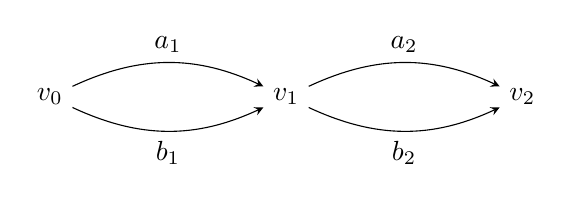
\begin{tikzpicture}[>=stealth]
\node (v0) at(0,0){$v_0$};\node(v1)at(3,0){$v_1$};\node(v2)at(6,0){$v_2$};
\draw[->](v0)to[bend left=25]node[above]{$a_1$}(v1);\draw[->](v0)to[bend right=25]node[below]{$b_1$}(v1);
\draw[->](v1)to[bend left=25]node[above]{$a_2$}(v2);\draw[->](v1)to[bend right=25]node[below]{$b_2$}(v2);
\end{tikzpicture}\par Figure 1. $2$-garland.\end{center}
Let $G:=(V,E)$ be a directed graph. Each edge $e\in E$ has the corresponding variable $x_e$, where $x_e=1$ indicates that a flow of size $1$ is going through an edge $e$. Let $u$ be an arbitrary, but fixed vertex of the graph.
The formula $\Flow_{G,u}$ consists of the following constraints written in CNF for all $v\in V$:
\[\sum_{e\in E:\st(e)=v}x_e-\sum_{e\in E:\en(e)=v}x_e\ge c(v),\]
where $e=(\st(e),\en(e))$ and $c:V\to\{0,1\}$ is a labeling function:
\[c(v)=0,\text{ for all }v\in V\setminus\{u\};\qquad c(u)=1.\]
This formulas states: for all vertices in the graph the flow is non-negative, and at least for one vertex it is strictly positive. It is easy to see that $\Flow_{G,u}$ is unsatisfiable. We omit index $u$ since in our applications it is an arbitrary vertex.
We use the most naive CNF encoding of these constraints. We represent each constraint separately. Consider a vertex $v\in V$ and a set of edges $E_v:=\{e_1,e_2,\ldots,e_s\}\subseteq E$ that are incident to $v$. Let $\rho_v:E_v\to\{0,1\}$ be an assignment that violates the constraint in $v$. In this case we add to the formula a clause $C$:
\[x_{e_1}^{1-\rho(x_{e_1})}\vee x_{e_2}^{1-\rho(x_{e_2})}\vee\cdots\vee x_{e_s}^{1-\rho(x_{e_s})},\]
and we also say that this assignment has a gap:
\[g(\rho_v):=c(v)-\sum_{e\in E:\st(e)=v}\rho_v(x_e)+\sum_{e\in E:\en(e)=v}\rho_v(x_e).\]
For our purpose we consider $\Flow_G$ based on expanders. To be precise, we start with a graph $G$ that is an $(n,\Delta,\alpha)$-expander, where $\Delta=\Theta(\log n)$ and $\alpha$ is some fixed constant, and replace each undirected edge by two directed edges (we say that these edges are dual). The exact value of $\Delta$ depends on a value of $k$.
\begin{result}{Remark 15}
We consider only proper partial assignments $\rho$ that satisfy the following property for all pairs of dual edges $(e,e')$:
\begin{itemize}\item $\rho(x_e)\in\{0,1\}$ iff $\rho(x_{e'})\in\{0,1\}$;
\item if $\rho(x_e)=1$ then $\rho(x_{e'})=0$.\end{itemize}
We also identify $\supp(\rho)$ with an undirected set of edges that are assigned by $\rho$.
\end{result}
To make the formula somewhat ``confusing'' for $(1,+k)$-BP, we would like to add more variables to clauses. These variables do not really affect the physical meaning of the formula, but make it hard for $(1,+k)$-BP to extract additional information from repetitions on paths. This transformation is sensitive to the exact CNF encoding of the constraints that is written above.
\begin{result}{Definition 16}
Let $G:=(V,E)$ be an undirected graph and $C_v$ be a subset of clauses corresponding to vertex $v$ in $\Flow_G$. Let $\eta_v^k:C_v\to\binom{E}{k}$ be a mapping, and $\eta^k:=\{\eta_v^k\mid v\in V\}$ be a family of such mappings. We define $\Flow_G^{\eta^k}$ the following way:
\begin{itemize}\item for each $v\in V$ we consider each $C\in C_v$;
\item we take $\eta_v^k(C)=\{e_1,\ldots,e_k\}$, which is a set of $k$ edges;
\item we replace $C$ by $2^{2k}$ clauses of the form:
\[C\vee\bigvee_i x_{s_i}^{a_i}\vee x_{s'_i}^{a'_i}\]
enumerated by $a_i,a'_i\in\{0,1\}$, where $i\in[k]$ and $s_i,s'_i$ are directed copies of the edge $e_i$.\end{itemize}
\end{result}
As described in the plan, at some point in the proof we would like to construct an assignment that leaves certain clauses (to which a certain set of variables was added) unsatisfied. For our purpose, we would like those clauses to ``strongly unsatisfy'' the condition in their vertices.
Let us describe the construction of $\eta^k$. Assume that $\Delta\ge50\cdot k\log n$. For each $v\in V$ we define $\eta_v$ independently. We will be interested in adding variables to clauses which correspond to large incoming flow.
\begin{enumerate}
\item Let us consider a set of clauses $\mathcal C$ that corresponds to $v$ and a proper partial assignment on edges incident to $v$ with gap equal to $\Delta/4+1$.
\item Note that $|\mathcal C|\ge\binom{\Delta}{\Delta/4}\ge4^{\Delta/4}\ge n^{4k}$. The first inequality holds since we can choose arbitrary $\Delta/4+1$ incoming edges to obtain the desired gap and set all other incident edges to zero.
\item There are at most $\binom{n\Delta}{k}\le(n\Delta e/k)^k\le n^{2k}$ different sets of $k$ edges. Hence we can choose a subset of $B\subseteq\mathcal C$ and define $\eta_v^k$ to be a bijection between $B$ and all possible choices of sets of $k$ edges.
\end{enumerate}
Note that the existence of $(1,+k)$-BP of size $S$ solving $\Search_{\Flow_G^{\eta^k}}$ (for any $\eta^k$) implies the existence of $(1,+k)$-BP of size $S$ solving $\Search_{\Flow_G}$.
\subsection*{4.1.1 Locally Consistent Assignments}
We need a notion of ``good assignments'', i.e. assignments that reduce $\Flow_G$ formulas to smaller, but ``equally hard'' instances.
Let $G:=(V,E)$ be a graph. A proper assignment $\rho$ $\delta$-satisfies a set of vertices $U\subseteq V$ iff for all $v\in U$ the following holds:
\begin{itemize}\item $\rho$ assigns all edges that are incident to $v$;
\item $\rho$ satisfies the constraint for $v$;
\item $\sum_{e\in E:\st(e)=v}\rho(x_e)\ge\delta\cdot\Delta$.\end{itemize}
We also say that a proper assignment $\rho$ is $(r,\delta,\beta)$-locally consistent iff there is a set of vertices $V_\rho$ of size at most $r$ such that:
\begin{itemize}\item $\rho$ $\delta$-satisfies $V_\rho$;
\item $(V\setminus V_\rho,E\setminus\supp(\rho))$ satisfies $(r,\beta)$-expansion property.\end{itemize}
\begin{result}{Remark 17}
If $\rho$ is an $(r,\delta,\beta)$-locally consistent assignment for some $\beta>0$, then $V_\rho$ is uniquely defined.
\end{result}
\begin{proof}
For the sake of contradiction assume that there are two candidates $A,B$. Wlog $A\setminus B\ne\emptyset$. Pick an arbitrary vertex $v\in A\setminus B$. Since $A$ satisfies the required properties, $\rho$ assigns all edges that are incident to $v$, which contradicts the fact that $(V\setminus B,E\setminus\supp(\rho))$ satisfies $(r,\beta)$-expansion property.
\end{proof}
\section*{Original Section 4.2: Proof of Theorem 2 (p.17:10)}
Let $G$ be an $(n,\Delta,\alpha)$-expander and $\eta^{k_0+1}$ be a mapping defined in section 4.1. In this section we prove an exponential lower bound on $\Search_{\Flow_G^{\eta^{k_0+1}}}$ for $(1,+k_0)$-BP. We assume that $n$ is large enough.
Let us fix some parameters:
\begin{itemize}
\item $\Delta:=100k_0\log n$ and $\Delta>200$;
\item $\alpha:=0.01$ is the second eigenvalue of the normalized adjacency matrix of $G$;
\item $r:=n/\Delta$ and $\beta:=0.96$ is the ``combinatorial expansion'' of the graph $G$;
\item $\beta':=0.95$ is an expansion parameter that we try to maintain after removing some vertices and edges from $G$;
\item $\nu_k:=(\tfrac14(\beta-\beta'))^{k+3}$ is a scaling factor that indicates the fraction of edges that we want to assign in our partial assignment.
\end{itemize}
Note that $r\ll(1-\beta-\alpha)n=0.03\cdot n$ and hence by Corollary 11 $G$ satisfies $(r,\beta)$-expansion property, hence we can use all combinatorial expansion properties and tools.
To formulate the induction hypothesis we need one more definition. Let $M\subseteq E$ and $\rho$ is a proper assignment. We say that $\rho$ is $\gamma$-minimal local consistent extension or (mlce) on $M$ iff:
\begin{itemize}\item $\rho$ is $(r,0.6,\gamma)$-locally consistent assignment;
\item $\supp(\rho)=M\cup E(V_\rho)$;
\item $|E(V_\rho,\overline{V_\rho})\setminus M|<\gamma\Delta|V_\rho|$.\end{itemize}
Informally we may think about it in the following way: after we assign edges from $M$ somehow, $\rho$ should assign also $V_\rho$ as a ``minimal'' set of vertices to take care of in order to be locally consistent.
Let $\varphi:=\Flow_G^{\eta^{k_0+1}}$. By induction on $k\le k_0$ we show the following statement. For all sets of edges $M\subseteq E$ of size at most $\nu_k\Delta r$ and all $\beta'$-mlce $\rho$ on $M$ any $(1,+k)$-BP for $\Search_{\varphi|_\rho}$ has size at least $2^{\frac{\nu_k}{4(k+1)^2}\Delta r}$.
Fix some $M,\rho,0\le k\le k_0$ and for the sake of contradiction assume that we have a $(1,+k)$-BP $D$ of size $2^{\frac{\nu_k}{4(k+1)^2}\Delta r}$ for $\Search_{\varphi|_\rho}$.

\section*{Original Section 4.2.1: Construction of the Garland (pp.17:11--12)}
To fulfill our plan of the proof, described at the beginning of the section, we start constructing the garland by obtaining an exponentially big set of paths with the corresponding assignments. Let us remind that $|M|\le\nu_k\Delta r$ and $\rho$ is $\beta'$-mlce on $M$.
We say that triple $(p,U_p,\sigma_p)$ is $\gamma$-good iff:
\begin{itemize}\item $p$ is a path from the root of the branching program;
\item $U$ is a subset of edges such that corresponding variables are queried on $p$, so-called ``branching variables'';
\item $\sigma_p$ is a partial assignment such that:
\begin{itemize}\item $\sigma_p$ extends $\rho\cup\tau_p$;
\item $\sigma_p$ is a $\gamma$-mlce on $M\cup U_p$;
\item $\sigma_p$ $0.8$-satisfies $V_{\sigma_p}\setminus V_\rho$,
\end{itemize}
where $\tau_p$ is an assignment that corresponds to $p$.\end{itemize}
We maintain the set of $\beta'$-good triples $\mathcal P$ and an auxiliary set $\mathcal S$ of triples that appear in the set $\mathcal P$ at some moment during the process. In the beginning of our construction $\mathcal P:=\{(\emptyset,\emptyset,\rho)\}$ and $\mathcal S:=\mathcal P$.
We repeat the following process while we have at least one triple $(p,U_p,\sigma_p)\in\mathcal P$ such that $|U_p|\le\nu_k\Delta r$.
Consider the triple described above. Let $v$ be the end of $p$ and $x_e$ be the variable asked in $v$.
\begin{enumerate}
\item If $x_e$ was queried on $p$ we stop the process. In this case we return ``Repetition'' and we remember the path $p$.
\item Erase the triple $(p,U_p,\sigma_p)$ from $\mathcal P$.
\item If $\sigma_p(x_e)\in\{0,1\}$, then we continue along the edge $x_e=\sigma_p(x_e)$. Consider a path $p'$ that is the extension of $p$ along this edge, $U_{p'}:=U_p$ and $\sigma_{p'}:=\sigma_p$. Put $(p',U_{p'},\sigma_{p'})$ into $\mathcal P$ and $\mathcal S$ and repeat the process from the beginning.
\item If $\sigma_p(x_e)=*$, then it is a ``branching node'', and we call this step a branching step.
\begin{enumerate}[label=\alph*.]
\item Let $p'$ be a path obtained by continuing $p$ along the edge $x_e=0$, and $p''$ be a path obtained by continuing $p$ along the edge $x_e=1$.
\item $U_{p'}:=U_p\cup e$, $U_{p''}:=U_p\cup e$.
\item $\tau':=\sigma_p\cup\{x_e=0,x_{e'}=0\}$, $\tau'':=\sigma_p\cup\{x_e=1,x_{e'}=0\}$, where $x_{e'}$ is a dual edge.
\item $(p',U_{p'},\tau')$ is $(\beta'-0.01)$-good triple. We extend an assignment $\tau'$ to make this triple $\beta'$-good. For the formal statement see Lemma 18. Here we describe an idea. Let $R\subseteq E$ be a set of edges that are unassigned by $\tau'$ (or $\tau''$), and $B\subseteq V\setminus V_{\sigma_p}$ be the maximal set of vertices that satisfies:
\[|B|\le r;\qquad |E(B,\overline B)\cap R|\le\beta'\Delta|B|.\]
Let $\kappa$ be an assignment on variables that correspond to edges in the set $E(B)\setminus\supp(\tau')$ such that $\tau'\cup\kappa$ $0.8$-satisfies the constraints for all $v\in B$. This assignment $\kappa$ always exists (and moreover it is independent of the value of $x_e$, but we do not use this fact).
\item We denote $\sigma_{p'}:=\tau'\cup\kappa$, $\sigma_{p''}:=\tau''\cup\kappa$ and put $(p',U_{p'},\sigma_{p'})$ and $(p'',U_{p''},\sigma_{p''})$ into $\mathcal P$ and into $\mathcal S$.
\end{enumerate}\end{enumerate}
To conclude the construction we want to show the following claims.
\begin{description}
\item[Repetition case.] In the first case of the proof (if we have a repetition) we can reduce the problem to a lower bound on $(1,+(k-1))$-BP.
\item[Correctness.] The branching step can be done and triples $(p',U_{p'},\sigma_{p'})$ and $(p'',U_{p''},\sigma_{p''})$ satisfy the required properties.
\item[Garland extraction.] Among these paths we can find an $k$-garland $(a,b)$ and a locally consistent extension of $\rho$.
\end{description}
\subsection*{4.2.1.1 Correctness}
We show that if we have a triple $(p,U_p,\tau_p)$ which is $\beta'$-good then after processing it with our algorithm we also put in our sets $\beta'$-good triples. Let us formulate the general Lemma that helps us with it.
\begin{result}{Lemma 18}
Let $(p,U_p,\sigma_p)$ and $(q,U_q,\sigma_q)$ be $0.9$-good triples. Then there is an assignment $\kappa$ such that:
\begin{itemize}\item for any $\gamma$ that is an instance of $\sigma_p\joint\sigma_q$ an assignment $\gamma\cup\kappa$ is a $\beta'$-mlce on $\supp(\sigma_p)\cup\supp(\sigma_q)$;
\item $|\supp(\gamma\cup\kappa)|\le\nu_{k-1}\Delta r$.\end{itemize}
Moreover if $p=q$ then triple $(p,U_p,\sigma_p\cup\kappa)$ is $\beta'$-good.
\end{result}
\begin{proof}
The proof was motivated by the closure technique developed in [1,3]. For the full version of the proof see Appendix A.
\end{proof}
If the branching step was not done, then we do not change $U$ and $\tau$, and we extend the path $p$ according to the assignment $\tau$ hence the triple remains $\beta'$-good. We are left with the branching step. Note that $(p',U_{p'},\tau')$ is $0.9$-good and we apply Lemma 18 to a pair composed of two identical triples $(p',U_{p'},\tau')$ and obtain $\kappa$ that satisfies the required properties.
\subsection*{4.2.1.2 Repetition case}
First let us note that if there is a repetition, then $k>0$. Suppose we found a repetition while considering a triple $(p,U_p,\sigma_p)$. The size of $M\cup U_p$ is at most $2\nu_k\Delta r$ and $\sigma_p$ is $\beta'$-mlce on $M\cup U_p$. Let $v$ be an end node of $p$. The program $D(v)|_{\sigma_p}$ is a $(1,+(k-1))$-BP for $\Search_{\Flow_G^{\eta^k}|_{\sigma_p}}$ by Lemma 8. Thus by induction hypothesis we have a lower bound of $2^{\frac{\nu_{k-1}}{4k^2}\Delta r}\ge2^{\frac{\nu_k}{4(k+1)^2}\Delta r}$ on the size of $D(v)|_{\sigma_p}$ and in this case we are done.
\subsection*{4.2.1.3 Garland extraction}
The following Lemma gives us a pair of triples $(p,U_p,\sigma_p),(q,U_p,\sigma_q)\in\mathcal P$ such that $(p,q)$ forms a $(k+1)$-garland.
\begin{result}{Lemma 19}
There are $(p,U_p,\sigma_p),(q,U_q,\sigma_q)\in\mathcal S$ such that $(p,q)$ forms a $(k+1)$-garland.
\end{result}
\begin{proof}For the proof see Appendix B.\end{proof}
To continue the proof we need some additional property that we can ``avoid repetitions'' in this garland. We say that there is a repetition in a garland $p=v_0p_1v_1p_2v_2p_3\ldots p_{k_0+1}v_{k_0+1}$ and $q=v_0q_1v_1q_2v_2q_3\ldots q_{k_0+1}v_{k_0+1}$ iff there is path in the garland, i.e. path $r$ of the form $v_0r_1v_1r_2v_2r_3\ldots r_{k_0+1}v_{k_0+1}$, such that some variable is queried more than one time on it, where $r_i\in\{p_i,q_i\}$.
Consider a path $r$ in our garland $(p,q)$ that contains a repetition and $r'\subseteq r$ the largest initial segment of $r$ without repetitions. Let $v$ be its end node. We apply Lemma 18 to triples $(p,U_p,\sigma_p),(q,U_q,\sigma_q)$, which gives us assignment $\kappa$, and choose a instance $\gamma$ of $\sigma_p\joint\sigma_q$ that is consistent with $\tau_{r'}$. Moreover, $|\supp(\gamma\cup\kappa)|\le\nu_{k-1}\Delta r$, and $\gamma\cup\kappa$ is a $\beta'$-mlce on $\supp(\sigma_p)\cup\supp(\sigma_q)$. Hence by Lemma 8 we can use the induction hypothesis for $(1,+k-1)$-BP $D(v)|_{\tau_{r'}}$ and formula $\varphi|_{\gamma\cup\kappa}$. The size of $D(v)|_{\tau_{r'}}$ is at least $2^{\frac{\nu_{k-1}}{4k^2}\Delta r}\ge2^{\frac{\nu_k}{4(k+1)^2}\Delta r}$.
For the rest of the proof we can assume that on any path $r$ of the form described above there are no repetitions.
\section*{Original Section 4.2.2: Unreachable Leaves (pp.17:13--14)}
Let us summarize what we have from the previous section. We created a pair of triples: $(p,U_p,\sigma_p)$ and $(q,U_q,\sigma_q)$ such that:
\begin{itemize}\item $(p,q)$ forms $(k_0+1)$-garland:
\[p=v_0p_1v_1p_2v_2p_3\ldots p_{k_0+1}v_{k_0+1};\quad q=v_0q_1v_1q_2v_2q_3\ldots q_{k_0+1}v_{k_0+1};\]
\item $(p,U_p,\sigma_p)$ and $(q,U_q,\sigma_q)$ are $\beta'$-good;
\item there are no repetitions on any path in the garland $(p,q)$.\end{itemize}
We use Lemma 18 for $(p,U_p,\sigma_p)$ and $(q,U_q,\sigma_q)$ and get an assignment $\kappa$. Let us fix an assignment $\gamma$ that is an instance of $\sigma_p\joint\sigma_q$ consistent with:
\begin{itemize}\item $\tau_p$;
\item values in $\sigma_q$ that do not contradict $\tau_p$\end{itemize}
and denote $\zeta:=\gamma\cup\kappa$. Note that, by construction:
\begin{itemize}\item $|\zeta|\le\nu_{k-1}\Delta r$;
\item $|\zeta|$ is $(r,0.6,\beta')$-locally consistent.\end{itemize}
In this section we describe a set of clauses that should be unreachable from the vertex $v_{k_0+1}$. Note that on each segment of a garland $(v_ip_iv_{i+1},v_iq_iv_{i+1})$ we query at least one variable in both assignments $\tau_p$ and $\tau_q$ and get the different values. Denote any variable that satisfies this property by $x_i$.
We remind that $\varphi:=\Flow_G^{\eta^{k_0+1}}$. Let $\mathcal D,\mathcal C$ be the subsets of clauses:
\[\mathcal D:=\{D\in\Flow_G\mid\text{for every }e\text{ that corresponds to some }x_i:e\in\eta^{k_0+1}(D)\}.\]
and
\[\mathcal C:=\{C\in\varphi\mid C\text{ is obtained from some }D\in\mathcal D\text{ by the amplification trick}\}.\]
For the sake of contradiction suppose that there is a path $s$ from $v_{k_0+1}$ such that:
\begin{itemize}\item $s$ is a consistent path and $\tau_s$ is consistent with $\zeta$ and hence $ps$ is also consistent;
\item $s$ ends in a clause $C\in\mathcal C$.\end{itemize}
Consider a family of paths $r_i:=v_0p_1v_1p_2v_2p_3\ldots p_{i-1}v_{i-1}q_iv_ip_{i+1}q_{i+1}p_{i+2}\ldots p_{k_0+1}v_{k_0+1}$, where $i\in[k_0+1]$. All paths $r_i$ are consistent since there are no repetitions in the garland $(p,q)$. Hence if $r_i$ is inconsistent with $s$ then on $s$ we requery some variable $x'_i$ from the segment $v_{i-1}q_iv_i$ and get an inconsistent value.
By construction, $\tau_s$ is consistent with $\zeta$, and $\zeta:=\gamma\cup\kappa$, where $\gamma$ is an instance of $\sigma_p\joint\sigma_q$. If $x'_i$ appeared in $v_{i-1}q_iv_i$, but not in $v_{i-1}p_iv_i$ (note that it cannot appear in any other segment of the garland, since there are no repetitions on the garland), then $(\sigma_p\joint\sigma_q)(x'_i)\in\{\sigma_q(x'_i),?\}$ and $\tau_p(x'_i)=*$ thus $\gamma(x'_i)=\sigma_q(x'_i)$ by the choice of $\gamma$. It follows that $\zeta(x'_i)=\sigma_q(x'_i)$ as well, and since $\tau_s$ is consistent with $\zeta$, we cannot obtain an inconsistent with $\tau_{q_i}$ value for $x'_i$ while requerying it. Hence $x'_i$ had appeared in $v_{i-1}p_iv_i$ as well, and on $s$ we requeried a variable from $v_{i-1}p_iv_i$ in consistent way. Moreover if all paths from some set $\{r_i\}_{i\in L}$ where $L\subseteq[k_0+1]$ are inconsistent with $s$ we requery at least $|L|$ variables from the path $p$ on the path $s$. Hence at least one of the paths $r_{i_0}$ is consistent with $s$, where $i_0\in[k_0+1]$ (or on the path $ps$ we requery at least $k_0+1$ variables).
\begin{result}{Remark 20}This is the only place there we use the property that there are no repetitions on the garland.\end{result}
Consider two paths $ps$ and $r_{i_0}s$:
\begin{itemize}\item these paths are consistent;
\item $\tau_{ps}(x_{i_0})\ne\tau_{r_{i_0}s}(x_{i_0})$.\end{itemize}
These properties imply that clause $C$ is not a legal answer for at least one these paths, and we have a contradiction with the assumption that there is a consistent path from $v_{k_0+1}$ to this clause. That gives us the desired description of leaves that should be unreachable for $v_{k_0+1}$.
To conclude the proof it remains to show that there should be a path from $v_{k_0+1}$ to at least one leaf marked by a clause $C\in\mathcal C$. We do it in the next section.

\section*{Original Section 4.2.3: Directing the Flow (pp.17:14--18)}
Let us remind that we deal with $\varphi:=\Flow_G^{\eta^{k_0+1}}$. To show that there is a path consistent with $\zeta$ from $v_{k_0+1}$ to a leaf with a label $C\in\mathcal C$ we show that $(\varphi\setminus\mathcal C)|_\zeta$ is satisfiable and hence there should be an extension of $\zeta$ that violates only clauses from $\mathcal C$.
\begin{result}{Remark 21}
If we do not care about assignment $\zeta$, the statement is trivial, since $\varphi$ is so-called minimally unsatisfiable formula (that becomes satisfiable after removing any clause). But $\zeta$ transforms our formula to ``heavily unsatisfiable'' formula, since $\zeta$ $0.6$-satisfies a lot of vertices (that was the crucial property that we used to create a garland).
\end{result}
Note that by construction of $\eta^{k_0+1}$ for each $v\in V$ there exists a clause $D\in\mathcal D$ that had originated from the constraint for $v$. For each $v$, we pick any such clause and denote it by $D_v$. We divide the rest of the proof into two parts.
\begin{enumerate}
\item ``Local part''. We find a carefully chosen large enough set of vertices $U\in V$ and an assignment $\tau\supseteq\zeta$ such that there is a set $V_\tau\supseteq(U\cup V_\zeta)$:
\begin{itemize}\item $(V\setminus V_\tau,E\setminus\supp(\tau))$ satisfies $(r,\beta')$-expansion property;
\item for all $v\in U$ the assignment $\tau$ violates $D_v$ and hence $\tau$ assigns all edges incident to $v$;
\item for all $v\in V_\tau\setminus U$ the assignment $\tau$ satisfies constraint for $v$.\end{itemize}
For this part we use the simplified version of technique used for the garland creation.
\item ``Global part''. By using Max-Flow Min-Cut Theorem we show that $\tau$ can be extended to total assignment that satisfies constraints for vertices whose constraints are neither satisfied nor falsified by $\tau$ yet.
\end{enumerate}
Since we satisfy all the constraints of $(\Flow_G\setminus\mathcal D)_\zeta$ this assignment also satisfies all constraints in $(\varphi\setminus\mathcal C)|_\zeta$ by the construction of the formula $\varphi$ (clauses of $\varphi$ are the weakened versions of the clauses $\Flow_G$).
Before we proceed with the proof let us define the ``overflow''.
\begin{result}{Definition 22}
The overflow introduced by a locally consistent assignment $\sigma$ is:
\[\of_\sigma:=1+\sum_{v\in V_\sigma}\left(\sum_{e\in E:\st(e)=v}x_e-\sum_{e\in E:\en(e)=v}x_e-c(v)\right).\]
\end{result}
Note that $\of_\zeta\le|\zeta|+1\le\nu_{k-1}\Delta r+1$.
\subsection*{4.2.3.1 Local part}
We start with the local part of the proof. In the beginning of our construction $U_0:=\emptyset$, $\tau_0:=\zeta$, $V_{\tau_0}:=V_\zeta$ and $i:=0$.
We repeat the following process while $\of_{\tau_i}>0$.
\begin{enumerate}
\item Choose a vertex $u_i$ that is untouched by $\tau_i$.
\item Let $\rho_{u_i}$ be an assignment to edges that are incident to $u_i$ such that $D_{u_i}$ is unsatisfied by $\rho_{u_i}$.
\item $\tau':=\tau_i\cup\rho_{u_i}$. Since $u_i$ is untouched by $\tau_i$ there is no intersection between $\rho_{u_i}$ and $\tau_i$.
\item Let $H_i\subseteq V\setminus V_{\tau_i}$ be the maximal set of vertices that satisfies:
\[|H_i|\le r;\qquad |E(H_i,\overline{H_i}\setminus\{u_i\})\setminus\supp(\tau_i)|\le\beta'\Delta|H_i|.\]
Let $\kappa_i$ be an assignment on variables that correspond to edges in the set $E(H)\setminus\supp(\tau')$ such that for all $v\in H_i$:
\[\sum_{e\in E:\st(e)=v}(\tau'\cup\kappa_i)(x_e)-\sum_{e\in E:\en(e)=v}(\tau'\cup\kappa_i)(x_e)=c(v).\]
\item $U_{i+1}:=U_i\cup\{u_i\}$, $\tau_{i+1}:=\tau'\cup\kappa_i$ and $V_{\tau_{i+1}}:=V_{\tau_i}\cup H_i\cup\{u_i\}$.
\item $i:=i+1$.
\end{enumerate}
Let $\ell$ be a number of iterations in this process. Let $U:=U_\ell$ and $\tau:=\tau_\ell$.
At first we give an upper bound on $\ell$. Since for all $i$ an assignment $\kappa_i$ exactly satisfies vertices in $H$, inclusion of $H$ into $V_\tau$ does not change the overflow. Assignment $\rho_{u_i}$ violates $D_{u_i}\in\mathcal D$ and by definition of $\eta^{k_0+1}$:
\[-\frac\Delta4-1\le\sum_{e\in E:\st(e)=u_i}\rho_{u_i}(x_e)-\sum_{e\in E:\en(e)=u_i}\rho_{u_i}(x_e)\le-\frac\Delta4.\]
Hence on each iteration $\of_{\tau_{i+1}}\le\of_{\tau_i}-\Delta/4$ and $|U|\le4|\zeta|/\Delta$ and $-\Delta/4-1\le\of_\tau\le0$.
\begin{result}{Lemma 23}
For all $i\le\ell$:
\begin{itemize}\item $\kappa_i$ exists;
\item $|V_{\tau_i}|\le\frac{1}{(\beta-\beta')\Delta}(\supp(\zeta)+\Delta|U_i|)$ and hence $|\tau_i|\le\frac{2}{\beta-\beta'}(|\supp(\zeta)|+\Delta|U_i|)$;
\item $(V\setminus V_{\tau_i},E\setminus\supp(\tau_i))$ satisfies $(r,\beta')$-expansion property.\end{itemize}
\end{result}
\begin{proof}This Lemma may be considered as simplified version of Lemma 18. For the proof see Appendix A.\end{proof}
To conclude the construction note that $\tau_i\le\tfrac{10}{4}\nu_{k-2}\Delta r\le\tfrac\Delta4 r$ for all $i\le\ell$ and we always can find the vertex untouched by $\tau_i$.
\begin{result}{Remark 24}This is the only place where we use that $r\le n/\Delta$.\end{result}
\subsection*{4.2.3.2 Global part}
Let $B:=V_\tau\setminus V_\zeta$. For the vertex $v\in V$ the overflow of $v$ is defined in the following way:
\[\of(v):=-\sum_{\substack{e\in\supp(\tau)\\\st(e)=u}}\tau(x_e)+\sum_{\substack{e\in\supp(\tau)\\\en(e)=u}}\tau(x_e)+c(v).\]
We want to create an auxiliary graph. Let $F^+:=\{v\in V\setminus V_\tau\mid\of(v)>0\}$ and $F^-:=\{v\in V\setminus V_\tau\mid\of(v)<0\}$. See Fig.2.
We define a graph $G':=(V',E')$ on vertices $V':=(V\setminus V_\tau)\cup\{s\}\cup\{t\}$, where $s$ is a source and $t$ is a sink. Edges $E'$ include four groups:
\begin{center}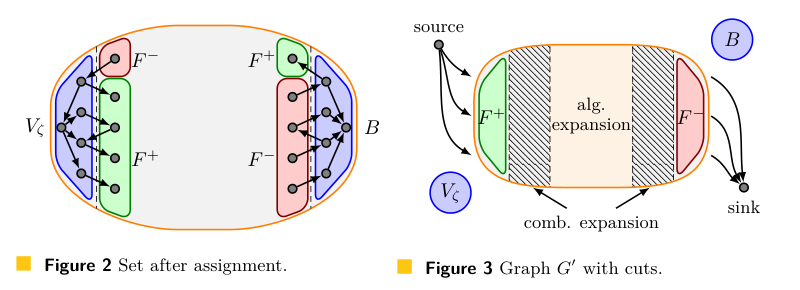
\includegraphics[width=.95\linewidth]{fig23.png}\end{center}
\begin{itemize}\item $E\setminus\supp(\tau)$;
\item we connect $s$ with all $v\in F^+$ by $\of(v)$ number of edges;
\item we connect $t$ with all $v\in F^-$ by $-\of(v)$ number of edges;
\item if $\of_\tau<0$ we choose an arbitrary set of vertices $S\in V\setminus V_\tau$ of size $|\of_\tau|$ and connect all $v\in S$ with $s$ by one more edge.\end{itemize}
See Fig.3.
\begin{result}{Remark 25}
\begin{enumerate}\item $\deg(s)=\deg(t)$;
\item If $A\subseteq V'$ then $E(\{s\},A)\le\Delta/4+1+\sum_{v\in A}\of(v)$ and $E(\{t\},A)=-\sum_{v\in A}\of(v)$.\end{enumerate}
\end{result}
\begin{proof}The first property follows from the construction of $\tau$ and the second one follows from definition of $G'$.\end{proof}
Let $f:=\deg(s)$. To conclude the proof we want to show that there is an $s$-$t$ flow in $G'$ of size $f$ (assuming that capacity of each edge is $1$) and that if this flow exists, then we have an extension of $\tau$ that satisfies $\Flow_G\setminus\mathcal D$. As we mention above together these facts imply that $(\Flow_G\setminus\mathcal D)|_\tau$ is satisfiable hence $(\Flow_G\setminus\mathcal D)|_\zeta$ is satisfiable and $(\varphi\setminus\mathcal C)|_\zeta$ is also satisfiable hence there is a path from $v_{k_0+1}$ to a leaf marked by some $C\in\mathcal C$ which is a contradiction with an existence of a garland and an assumption about size of the branching program.
We start with the second part. Suppose that we have a flow of size $f$. Fix the flow that achieves this value. We define a total proper assignment $\sigma\supseteq\tau$ in the natural way. Consider an edge $e\in E'\cup E$ and $a=(u,v)$, $a'=(v,u)$ its directed copies. If there is a flow on the edge $e$:
\begin{itemize}\item from $u$ to $v$ then $x_a=1$ and $x_{a'}=0$;
\item from $v$ to $u$ then $x_a=0$ and $x_{a'}=1$.\end{itemize}
otherwise we set $x_a=0$ and $x_{a'}=0$.
Note that $f=\deg(s)$ hence we use all edges that connect $s$ with other vertices to push the flow. That implies for all $v\in V\setminus V_\tau$:
\[\sum_{\substack{e\in\supp(\sigma)\setminus\supp(\tau)\\\st(e)=v}}\sigma(x_e)+\sum_{\substack{e\in\supp(\sigma)\setminus\supp(\tau)\\\en(e)=v}}\sigma(x_e)=|E(s,v)|=\of(v)\]
and hence
\[\sum_{e\in E:\st(e)=v}\sigma(x_e)+\sum_{e\in E:\en(e)=v}\sigma(x_e)=c(v).\]
and constraints for all vertices in $V\setminus V_\tau$ are satisfied, but $\tau$ itself satisfied all constraints in $\Flow_G\setminus\mathcal D$ that correspond to vertices in $V_\tau$. Altogether it says that $\sigma$ satisfies all constraints in $\Flow_G\setminus\mathcal D$ as desired.
It remains to show that we have an $s$-$t$ flow of size $f$ in $G'$. To do it we use the Max-Flow Min-Cut Theorem and show that minimal $s$-$t$ cut has size $f$. Consider such a cut $(S,T)$, where $S,T$ are disjoint subsets of $V'$ such that $s\in S$ and $t\in T$. We consider two cases:
\begin{itemize}\item either $S$ or $T$ is small enough, then we use the $(r,\beta')$-expansion property that we have after removing $\supp(\tau)$ and $V_\tau$ from $G$;
\item $S$ and $T$ are large enough, then we use the Mixing Lemma to show that even removing $\supp(\tau)$ from $G$ cannot destroy balanced cuts.\end{itemize}
see Fig.3.
\begin{center}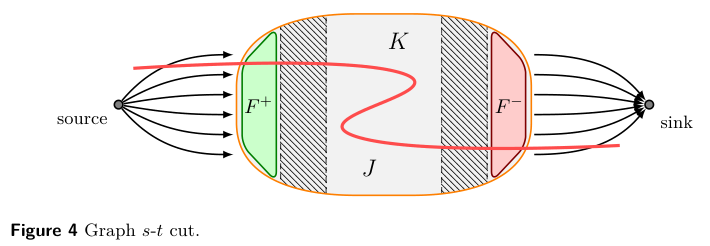
\includegraphics[width=.8\linewidth]{fig4.png}\end{center}
Consider an arbitrary $s$-$t$ cut $S\cup T$. Let $J:=S\setminus\{s\}$ and $K:=T\setminus\{t\}$ (see Fig.4). Consider the following cases.
\begin{enumerate}
\item If $J=\emptyset$ or $K=\emptyset$ then size of $(S,T)$ cut equals $\deg(s)$ or $\deg(t)$ respectively and we are done.
\item $0<|J|\le r$ or $0<|K|\le r$. Wlog assume that $|J|\le r$. Note that:
\[E_{G'}(S,T)=E_{G'}(\{s\},K)+E_{G'}(\{t\},J)+E_{G'}(J,K).\]
$E_{G'}(\{s\},K)=\sum_{v\in F^+\cap K}\of(v)$, so by Remark 25 to give a lower bound on the size of cut it is enough to show that $E_{G'}(J,K)\ge\Delta/4+1+\sum_{v\in F^+\cap J}\of(v)$. But $(V\setminus V_\tau,E\setminus\supp(\tau))$ satisfies $(r,\beta')$-expansion property. Hence
\begin{itemize}\item for all $v\in V\setminus V_\tau$: $|\of(v)|\le0.1\cdot\Delta$;
\item $|E_{G'}(J,K)|\ge0.9\cdot\Delta|J|$,\end{itemize}
that implies that $|E_{G'}(J,K)|-\Delta/4-1\ge2\sum_{v\in F^+\cap J}\of(v)$.
\item $|J|>r$, $|K|>r$. Wlog assume that $|J|\le|K|$. By Mixing Lemma:
\begin{align*}
|E_G(J,\overline J)|&=\Delta|J|-E_G(J,J)\ge\Delta|J|-\frac\Delta n|J|^2-\alpha\Delta|J|\\
&\ge\Delta|J|-|J|-\alpha\Delta|J|\ge0.9\cdot\Delta r,
\end{align*}
and
\[|E_{G'}(J,K)|\ge|E_G(J,\overline J)|-|\supp(\tau)|\ge0.6\cdot\Delta r.\]
On the other hand:
\begin{align*}
f&=\sum_{v\in F^+}\of(v)\\
&=\sum_{v\in F^+}\left(-\sum_{\substack{e\in\supp(\tau)\\\st(e)=u}}\tau(x_e)+\sum_{\substack{e\in\supp(\tau)\\\en(e)=u}}\tau(x_e)+c(v)\right)\\
&\le|\supp(\tau)|\le\frac\Delta4 r.
\end{align*}
\end{enumerate}
Hence in all cases $(S,T)$ has size at least $f$ which by Max-Flow Min-Cut Theorem implies the existence of flow in $G'$ of size at least $f$. That as mentioned above implies the desired lower bound on the size of branching program.

\section*{Original Appendix A: Missed Lemmas (pp.17:21--25)}
\subsection*{A.1 Lemma 18}
At first we prove an auxiliary Lemma.
\begin{result}{Lemma 28}
If $G:=(V,E)$ satisfies $(r,a)$-expansion property, $M\subseteq E$, and $S\subseteq V$ of size at most $r$, such that $|E(S,\overline S)\setminus M|\le b\Delta|S|$ then $|S|\le\frac{|M|}{(a-b)\Delta}$.
\end{result}
\begin{proof}
The size of $S$ is at most $r$, hence:
\[b\Delta|S|\ge|E(S,\overline S)\setminus M|\ge a\Delta|S|-|M|.\]
Thus $|S|\le\frac{|M|}{(a-b)\Delta}$.
\end{proof}
\begin{result}{Lemma A.1 (18)}
Let $(p,U_p,\sigma_p)$ and $(q,U_q,\sigma_q)$ be $0.9$-good triples. Then there is an assignment $\kappa$ such that:
\begin{itemize}\item for any $\gamma$ that is an instance of $\sigma_p\joint\sigma_q$ an assignment $\gamma\cup\kappa$ is a $\beta'$-mlce on $\supp(\sigma_p)\cup\supp(\sigma_q)$;
\item $|\supp(\gamma\cup\kappa)|\le\nu_{k-1}\Delta r$.\end{itemize}
Moreover if $p=q$ then triple $(p,U_p,\sigma_p\cup\kappa)$ is $\beta'$-good.
\end{result}
\begin{proof}
Let $S:=V_{\sigma_p}\cup V_{\sigma_q}$, $E_\sigma:=\supp(\sigma_p)\cup\supp(\sigma_q)$ and $B\subseteq V\setminus S$ be the maximal set of vertices that satisfies:
\[|B|\le r;\qquad |E(B,\overline B)\setminus E_\sigma|\le\beta'\Delta|B|.\]
At first we give an upper bound on the size of set $B$.
Partial assignment $\sigma_p$ is $0.9$-mlce on $M\cup U_p$. $\beta'\Delta|V_{\sigma_p}|\ge|E(V_{\sigma_p},\overline{V_{\sigma_p}})\setminus(M\cup U_p)|$ and by Lemma 28
\[|V_{\sigma_p}|\le\frac{|M\cup U_p|}{(\beta-\beta')\Delta}\le2\frac{\nu_k}{\beta-\beta'}r\le\tfrac12\nu_{k-1}r.\]
By analogy the same holds for $V_{\sigma_q}$.
The equality $E(B,\overline B)\cap E_\sigma=E(B,S)\cup(E(B)\cap|M\cup U_p\cup U_q|)$ together with $|E(B,\overline B)\setminus E_\sigma|\le\beta'\Delta|B|$ implies:
\[(1-\beta')\Delta|B|-|M\cup U_p\cup U_q|\le|E(B,S)|.\]
By Mixing Lemma:
\[|E(B,S)|\le\frac\Delta n|B||S|+\alpha\Delta\sqrt{|S||B|}.\]
For the sake of contradiction assume that $|B|\ge|S|$ thus:
\[|E(B,S)|\le\frac\Delta n|B||S|+\alpha\Delta|B|.\]
Altogether:
\[(1-\beta')\Delta|B|\le\frac{\Delta r}{n}\nu_{k-1}|B|+\alpha\Delta|B|+3\nu_k\Delta r\le2\alpha\Delta|B|,\]
that contradicts the choice of $\alpha$ and $\beta'$, hence $|B|\le|S|\le\nu_{k-1}r$.
At first we show that $(V\setminus(S\cup B),E\setminus(E_\sigma\cup E(B)))$ satisfies $(r,\beta')$-expansion property. By contradiction, suppose that there is a set $B'\subseteq V\setminus(S\cup B)$ of size at most $r$ such that
\[|E(B',\overline{B'})\setminus(E_\sigma\cup E(B))|<\beta'\Delta|B'|.\]
Again by Lemma 28 we conclude that:
\[|B'|\le\frac{|M\cup U_p\cup U_q|+\Delta|S\cup B|}{(\beta-\beta')\Delta}\le\nu_{k-1}r+\tfrac12r\le\tfrac34r.\]
But it implies that $|B\cup B'|\le r$, moreover:
\begin{align*}
|E(B\cup B',\overline{B\cup B'})\setminus E_\sigma|&\le\beta'\Delta|B|+\beta'\Delta|B'|\\
&=\beta'\Delta|B\cup B'|.\qquad\text{$B$ and $B'$ are disjoint}
\end{align*}
That contradicts the choice of $B$.
Now we find a proper assignment $\kappa$ on the $E(B)\setminus E_\sigma$ such that for all $v\in B$:
\[\sum_{e\in E:\st(e)=v}x_e\ge0.8\cdot\Delta.\]
Since $\sigma_p$ is an $(r,0.6,0.9)$-locally consistent assignment, then $(V\setminus V_{\sigma_p},E\setminus\supp(\sigma_p))$ satisfies $(r,0.9)$-expansion property. By analogy we have the same property for $\sigma_q$ that implies: $(V\setminus S,E\setminus E_\sigma)$ satisfies $(r,0.8)$-expansion property. Indeed, consider a set $C\subseteq V\setminus S$ of size at most $r$:
\begin{align*}
|E(C,\overline C)\setminus E_\sigma|&=|E(C,\overline C)|-|E(C,\overline C)\cap E_\sigma|\\
&\ge|E(C,\overline C)|-|E(C,\overline C)\cap\supp(\sigma_p)|-|E(C,\overline C)\cap\supp(\sigma_q)|\\
&=|E(C,\overline C)\setminus\supp(\sigma_p)|-0.1\cdot\Delta|C|\\
&\ge0.8\cdot\Delta|C|.
\end{align*}
By Proposition 12 there is an enumeration of vertices in $B$: $v_1,v_2,\ldots,v_{|B|}\in B$ and a sequence $R_1,\ldots,R_{|B|}\subseteq(E(B)\setminus E_\sigma)$ such that:
\[R_i=E(\{v_i\},V\setminus\{v_1,v_2,\ldots,v_i\})\setminus E_\sigma;\quad |R_i|\ge0.8\Delta.\]
We define $\kappa$ in the following way:
\begin{itemize}\item for an $e\in R_i$ we assign corresponding variables to direct the flow outside of the vertex $v_i$ (i.e. if $e'$ is a directed copy of $e$ that goes outside of $v_i$ we set $x_{e'}$ to $1$ and set the dual edge to $0$);
\item for all loops inside the set $B$ we assign corresponding variables to $0$.\end{itemize}
Let $\gamma$ be an instance of $\sigma_p\joint\sigma_q$, $\zeta:=\gamma\cup\kappa$ and $V_\zeta:=S\cup B$. We have already shown that the graph $(V\setminus V_\zeta,E\setminus\supp(\zeta))$ satisfies $(r,\beta')$-expansion property. We want to show that vertices in $V_\zeta$ are $0.6$-satisfied by $\zeta$. Consider four cases.
\begin{enumerate}
\item $v\in V_\rho$. Both assignments $\sigma_p$ and $\sigma_q$ extend an assignment $\rho$ hence $\gamma$ agreed with both assignments on edges incident to $V_\rho$. Thus $\gamma$ $0.6$-satisfies $v$.
\item $v\in V_{\sigma_p}\setminus V_\rho$. Let $E_v$ be a set of edges that are incident to $v$. At least $0.8\cdot\Delta$ of those edges carry outgoing flow from $v$ in $\sigma_p$. Denote those edges as $E_{\sigma_p}$.
If $v\notin V_{\sigma_q}$ then $\sigma_q$ may assign at most $0.1\cdot\Delta$ edges in $E_v$. That means that in $\gamma$ at least $0.7\cdot\Delta$ edges from $E_{\sigma_p}$ still carry outgoing flow from $v$.
If $v\in V_{\sigma_q}$ then $\sigma_p$ and $\sigma_q$ both $0.8$-satisfy $v$. Let $E_{\sigma_q}\subseteq E_v$ be the set of edges that carry outgoing flow from $v$ in $\sigma_q$. Then $E_{\sigma_p}\cap E_{\sigma_q}\ge0.6\cdot\Delta$, and all those edges carry outgoing flow from $v$ in $\gamma$.
Note that if $\sigma_p=\sigma_q$, then we $0.8$-satisfy $v$.
\item $v\in V_{\sigma_p}\setminus V_\rho$. By analogy with the previous case.
\item $v\in B$. We direct the flow on at least $0.8\cdot\Delta$ edges from $E_v$ outside of $v$ hence $\kappa$ $0.8$-satisfies $v$.
\end{enumerate}
By construction $V_\zeta:=V_{\sigma_p}\cup V_{\sigma_q}\cup B$ hence $|V_\zeta|\le\nu_{k-1}r$ and $|\supp(\zeta)|\le\nu_{k-1}r$. In order to check that $\zeta$ is $\beta'$-mlce note that:
\[|E(B,\overline B)\setminus E_\sigma|\le\beta'\Delta|B|\le\beta'\Delta|V_\zeta|,\]
but
\[|E(B,\overline B)\setminus E_\sigma|=|E(V_\zeta,\overline{V_\zeta})\setminus E_\sigma|\]
since $\sigma_p$ and $\sigma_q$ together assign all edges that are incident to $V_{\sigma_p}\cup V_{\sigma_q}$. Thus:
\[|E(V_\zeta,\overline{V_\zeta})\setminus E_\sigma|\le\beta'\Delta|V_\zeta|\]
that concludes the proof.
In case of $(p,U_p,\sigma_p)=(q,U_q,\sigma_q)$ it remains to show that $\zeta$ is $\beta'$-mlce on $M\cup U_p$. Again we note that:
\[|E(B,\overline B)\setminus E_\sigma|\le\beta'\Delta|B|,\]
and also
\[|E(V_{\sigma_p},\overline{V_{\sigma_p}})\setminus E_\sigma|\le\beta'\Delta|V_{\sigma_p}|,\]
hence
\begin{align*}
|E(V_{\sigma_p}\cup B,\overline{V_{\sigma_p}\cup B})\setminus E_\sigma|
&\le\beta'\Delta(|V_{\sigma_p}|+|B|)\\
&\le\beta'\Delta|V_{\sigma_p}\cup B|,
\end{align*}
where the last inequality holds since $B$ and $V_{\sigma_p}$ are disjoint, that concludes the proof.
\end{proof}
\subsection*{A.2 Lemma 23}
\begin{result}{Lemma A.2 (23)}
For all $i\le\ell$:
\begin{itemize}\item $\kappa_i$ exists;
\item $|V_{\tau_i}|\le\frac{1}{(\beta-\beta')\Delta}(\supp(\zeta)+\Delta|U_i|)$ and hence $|\tau_i|\le\frac{2}{\beta-\beta'}(|\supp(\zeta)|+\Delta|U_i|)$;
\item $(V\setminus V_{\tau_i},E\setminus\supp(\tau_i))$ satisfies $(r,\beta')$-expansion property.\end{itemize}
\end{result}
\begin{proof}
We show by induction on $i$ that:
\begin{itemize}\item $(V\setminus V_{\tau_i},E\setminus\supp(\tau_i))$ satisfies $(r,\beta')$-expansion property;
\item $|E(V_{\tau_i},\overline{V_{\tau_i}})\setminus(\supp(\zeta)\cup E(U_i))|<\beta'\Delta|V_{\tau_i}|$;
\item $|V_{\tau_i}|\le\frac{1}{(\beta-\beta')\Delta}(\supp(\zeta)+\Delta|U_i|)$ and hence $|\tau_i|\le\frac{2}{\beta-\beta'}(|\supp(\zeta)|+\Delta|U_i|)$.\end{itemize}
Assignment $\tau_0$ is $\zeta$ and $\zeta$ is $(r,0.6,\beta')$-locally consistent, in particular, $(V\setminus V_\zeta,E\setminus\supp(\zeta))$ satisfies $(r,\beta')$-expansion property and $E(V_\zeta,\overline{V_\zeta})\setminus\supp(\zeta))=\emptyset$.
By definition of $H_i$:
\[\beta'\Delta|H_i|>|E(H_i,\overline{H_i}\setminus\{u_i\})\setminus\supp(\tau_i)|\ge|E(H_i,\overline{H_i})\setminus(\supp(\tau_i)\cup E(H_i,\{u_i\}))|\]
and by Lemma 28
\[|H_i|\le\frac{|\supp(\tau_i)\cup E(H_i,u_i)|}{(\beta-\beta')\Delta}\le\frac{|\supp(\tau_i)\cup E(H_i,u_i)|}{(\beta-\beta')\Delta}\le\tfrac12\nu_{k-2}(r+1).\]
Hence $|H_i\cup V_{\tau_i}\cup\{u_i\}|\le r$ that together with:
\begin{align*}
&|E(H_i\cup V_{\tau_i},\overline{H_i\cup V_{\tau_i}})\setminus(\supp(\zeta)\cup E(U_{i+1}))|\\
&\le |E(V_{\tau_i},\overline{H_i\cup V_{\tau_i}})\setminus(\supp(\zeta)\cup E(U_{i+1}))|\\
&\quad+|E(H_i,\overline{H_i})\setminus(\supp(\zeta)\cup E(U_{i+1})\cup E(V_{\tau_i})|\\
&\le\beta'\Delta|V_{\tau_i}|+\beta'\Delta|H_i|\le\beta'\Delta|H_i\cup V_{\tau_i}|\le\beta'\Delta|H_i\cup V_{\tau_i}\cup\{u_i\}|
\end{align*}
implies $|V_{\tau_{i+1}}|=|H_i\cup V_{\tau_i}\cup\{u_i\}|\le\frac{1}{(\beta-\beta')\Delta}(|\supp(\zeta)|+\Delta|U_{i+1}|)$ by Lemma 28. Also $|\tau_{i+1}|\le\frac{2}{\beta-\beta'}(|\supp(\zeta)|+\Delta|U_{i+1}|)$ since by construction $\tau_{i+1}$ assigns only edges in $\supp(\zeta)\cup E(U_i\cup V_{\tau_{i+1}})$.
Now we show that a graph $(V\setminus V_{\tau_{i+1}},E\setminus\supp(\tau_{i+1}))$ satisfies $(r,\beta')$-expansion property. For the sake of contradiction assume that there is a set $S\subseteq V\setminus V_{\tau_{i+1}}$ of size at most $r$ such that: $E(S,\overline S)\setminus\supp(\tau_{i+1})\le\beta'\Delta|B|$.
By Lemma 28 $|S|\le\frac{|\supp(\tau_{i+1})|}{(\beta-\beta')\Delta}\le\tfrac12\nu_{k-2}(r+1)$. Hence $|H_i\cup S|\le r$ that together with:
\begin{align*}
&E(H_i\cup S,\overline{H_i\cup S}\setminus\{u_i\})\setminus\supp(\tau_i)|\\
&\le E(H_i,\overline{H_i\cup S}\setminus\{u_i\})\setminus\supp(\tau_i)|+E(S,\overline{H_i\cup S}\setminus\{u_i\})\setminus\supp(\tau_i)|\\
&\le\beta'\Delta|H_i|+\beta'\Delta|S|=\beta'\Delta|H_i\cup S|
\end{align*}
contradicts the choice of $H_i$.
To conclude the proof we have to show the existence of $\kappa_i$. Note that $(V\setminus V_{\tau_i},E\setminus\supp(\tau_i))$ satisfies $(r,\beta')$-expansion property. Consider an arbitrary set $B\subseteq V\setminus(V_{\tau_i}\cup\{u_i\})$ of size at most $r$:
\[|E(B,\overline B)\setminus(\supp(\tau_i)\cup E(\{u_i\}))|\ge\beta'\Delta|B|-E(B,\{u\}).\]
By Mixing Lemma:
\[|E(B,\{u\})|\le\frac\Delta n|B|+\alpha\Delta\sqrt B\le0.05\cdot\Delta|B|,\]
and hence
\[|E(B,\overline B)\setminus(\supp(\tau_i)\cup E(\{u_i\}))|\ge0.9\cdot\Delta|B|\]
and graph $(V\setminus V_{\tau_i}\setminus\{u_i\},E\setminus\supp(\tau_i))$ satisfies $(r,0.9)$-expansion property.
By Proposition 12 there is an enumeration of vertices in $H_i$: $v_1,v_2,\ldots,v_{|H_i|}\in H_i$ and a sequence $R_1,\ldots,R_{|H_i|}\subseteq E(H_i)\setminus(\supp(\tau_i)\cup E(\{u_i\}))$ such that:
\[R_k=E(\{v_k\},V\setminus\{v_1,v_2,\ldots,v_k\})\setminus(\supp(\tau_i)\cup E(\{u_i\}));\qquad |R_i|\ge0.9\cdot\Delta.\]
We define $\kappa_i$ for vertices $v_1,\ldots,v_{H_i}$ step by step, such that $\kappa_i$ on $E(v_k)$ satisfies the constraint:
\[\sum_{e\in E:\st(e)=v_k}(\tau'\cup\kappa_i)(x_e)-\sum_{e\in E:\en(e)=v_k}(\tau'\cup\kappa_i)(x_e)=c(v_k).\]
Since we have an access to the $0.9\cdot\Delta$ edges and others are already assigned, we can always choose the right values (loops are always assigned to zero).
\end{proof}
\section*{Original Appendix B: Garland in the Paths (p.17:25)}
\begin{result}{Lemma B.1 (19)}
There are $(p,U_p,\sigma_p),(q,U_q,\sigma_q)\in\mathcal S$ such that $(p,q)$ forms a $(k+1)$-garland.
\end{result}
\begin{proof}
Note that we can describe elements in $\mathcal P$ by a sequence of bits of size $s:=\nu_k\Delta r$. Each bit of this sequence describes an assignment for an edge $e$ that we choose on ``branching step''. From the construction it follows that different sequences generate different paths in the branching program and hence different elements of $\mathcal P$.
Let $s_k:=\lfloor s/(k+1)\rfloor$. We construct our garland by the iterative algorithm. After $i$-th iteration we have a set $S_i$ of sequences of size $is_k$ such that any two of the corresponding paths form $i$-garland and all paths end in the same node. The size of $S_i$ will be at least $\exp[s_k-\frac{i}{2k}s_k]$ for all $1\le i\le k+1$.
\begin{enumerate}
\item For $i=1$ consider all possible strings of length $s_k$ and paths that correspond to them. The branching program has size at most $2^{s_k/(2k)}$, hence there exists a node such that at least $2^{s_k(2k-1)/(2k)}$ paths end there. The set $S_1$ consists of all corresponding sequences.
\item For the step $i$, $2\le i\le k+1$, we consider all sequences in $S_{i-1}$. Let $v$ be the end node of all paths corresponding to sequences in the set. To each sequence $s\in S_{i-1}$ we append a string $u_s$ of $s_k$ bits in such a way that for any pair $r,r'\in S_{i-1}$ paths that corresponds to $ru_r$ and $r'u_{r'}$ differ at some node after $v$. Since $2^{s_k}\ge|S_{i-1}|$, it is possible to do this.
For the resulting sequences, we consider the set of the corresponding paths. The set of paths has size at least $2^{s_k(2k-i+1)/(2k)}$, and the size of the program is at most $2^{s_k/(2k)}$. Hence there exists a node such that $2^{s_k(2k-i)/(2k)}$ paths end there. Let $S_i$ be the set of sequences corresponding to those paths.
\end{enumerate}
After $k+1$ steps we have a set $S_{k+1}$, $|S_{k+1}|\ge2$, such that any two sequences in it correspond to a $(k+1)$-garland.
\end{proof}

\begin{thebibliography}{12}
\bibitem[1]{source1} Michael Alekhnovich, Eli Ben-Sasson, Alexander A. Razborov, and Avi Wigderson. Pseudorandom generators in propositional proof complexity. \emph{SIAM J. Comput.}, 34(1):67--88, 2004. doi:10.1137/S0097539701389944.
\bibitem[3]{source3} Michael Alekhnovich and Alexander A. Razborov. Lower bounds for polynomial calculus: Non-binomial case. \emph{Proceedings of the Steklov Institute of Mathematics}, 242:18--35, 2003. Preliminary version in FOCS '01.
\bibitem[4]{source4} Noga Alon and Fan R. K. Chung. Explicit construction of linear sized tolerant networks. \emph{Discret. Math.}, 72(1-3):15--19, 1988. doi:10.1016/0012-365X(88)90189-6.
\bibitem[8]{source8} L. R. Ford and D. R. Fulkerson. Maximal flow through a network. \emph{Canadian Journal of Mathematics}, 8:399--404, 1956. doi:10.4153/CJM-1956-045-5.
\bibitem[9]{source9} Konstantinos Georgiou, Avner Magen, and Madhur Tulsiani. Optimal sherali-adams gaps from pairwise independence. In Irit Dinur, Klaus Jansen, Joseph Naor, and Jos\'e Rolim, editors, \emph{Approximation, Randomization, and Combinatorial Optimization. Algorithms and Techniques}, pages125--139, Berlin, Heidelberg, 2009. Springer Berlin Heidelberg.
\end{thebibliography}
\end{document}
